\chapter{Experiments}



\section{Remaining Plots}
	\label{app:remainingPlots}

	In this section we put all plots referenced in~\autoref{sec:results} that where not directly in that section as they do not add much new information. List of plots:
	\begin{itemize}
		\item Gym cartpole, 1-dimensional latent, rollout with confidence:~\autoref{fig:cartpoleRolloutL02Appendix}
		\item Gym cartpole, 10-dimensional latent, rollout without confidence:~\autoref{fig:cartpoleRolloutL10Appendix}
		\item Gym cartpole, 31-dimensional latent, rollout without confidence:~\autoref{fig:cartpoleRolloutL14Appendix}
	\end{itemize}

	\begin{figure}
		\centering
		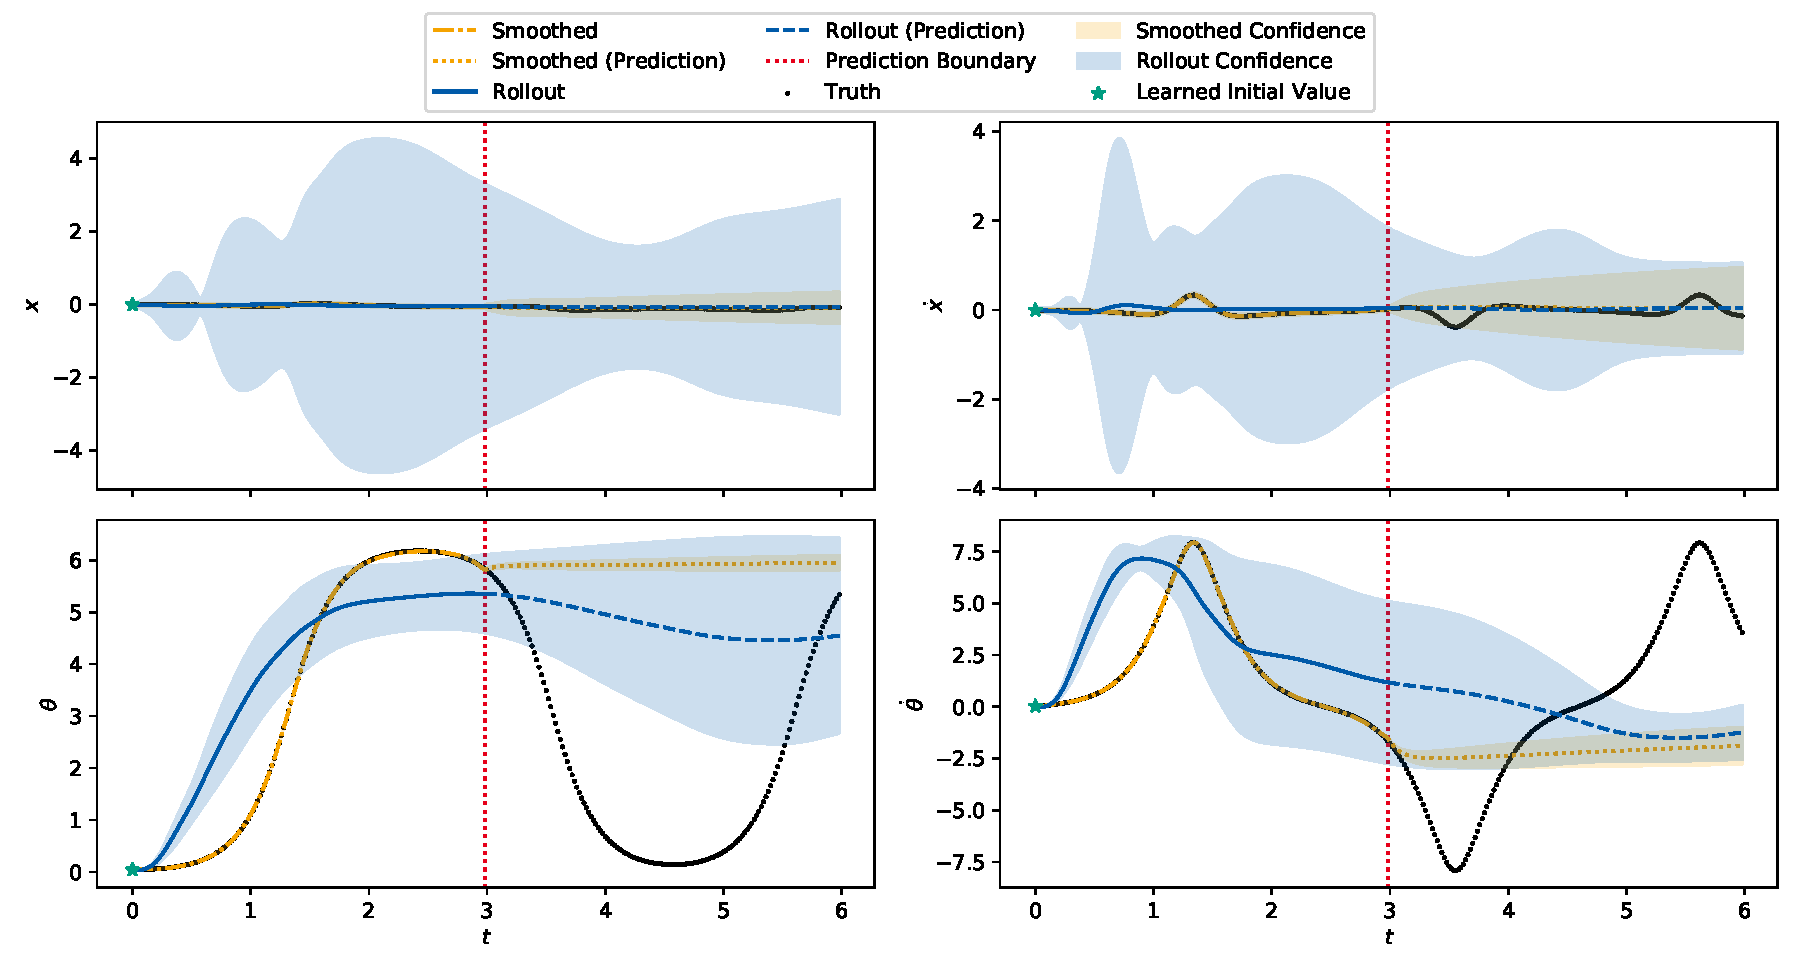
\includegraphics[width=\linewidth]{figures/results/cartpole-gym/run-latent-dim-02/rollout-observations-N0.pdf}
		\caption{This plot shows the same data as in~\autoref{fig:cartpoleRolloutL02}, but with the confidence shown. As the confidence is quite low, this plot is hard to interpret which is the reason why we removed the confidence plot in the first place.}
		\label{fig:cartpoleRolloutL02Appendix}
	\end{figure}

	\begin{figure}
		\centering
		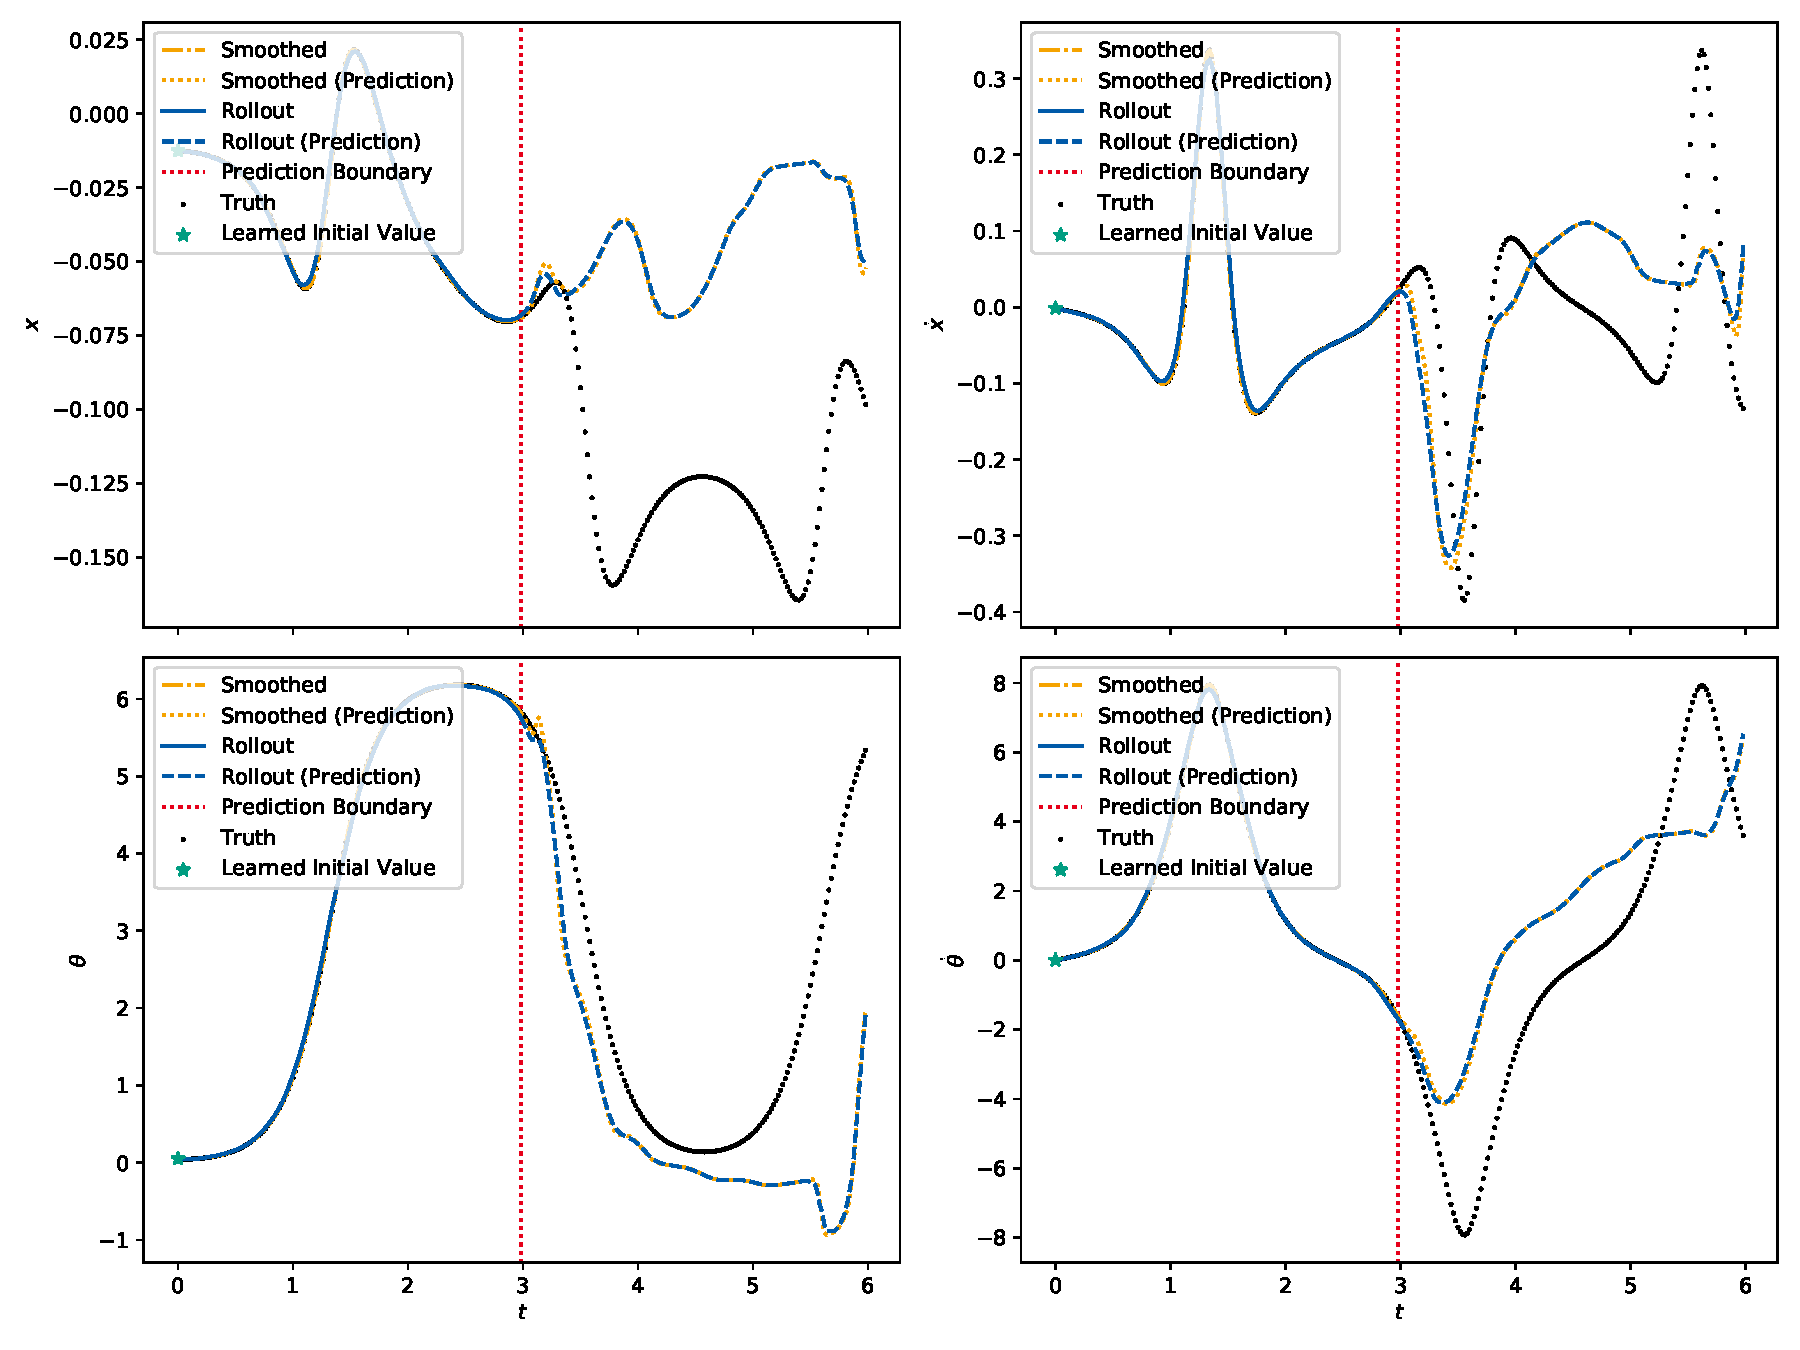
\includegraphics[width=\linewidth]{figures/results/cartpole-gym/run-latent-dim-10/without-confidence/rollout-observations-N0.pdf}
		\caption{This plot shows the same data as in~\autoref{fig:cartpoleRolloutL10}, but without the confidence shown.}
		\label{fig:cartpoleRolloutL10Appendix}
	\end{figure}

	\begin{figure}
		\centering
		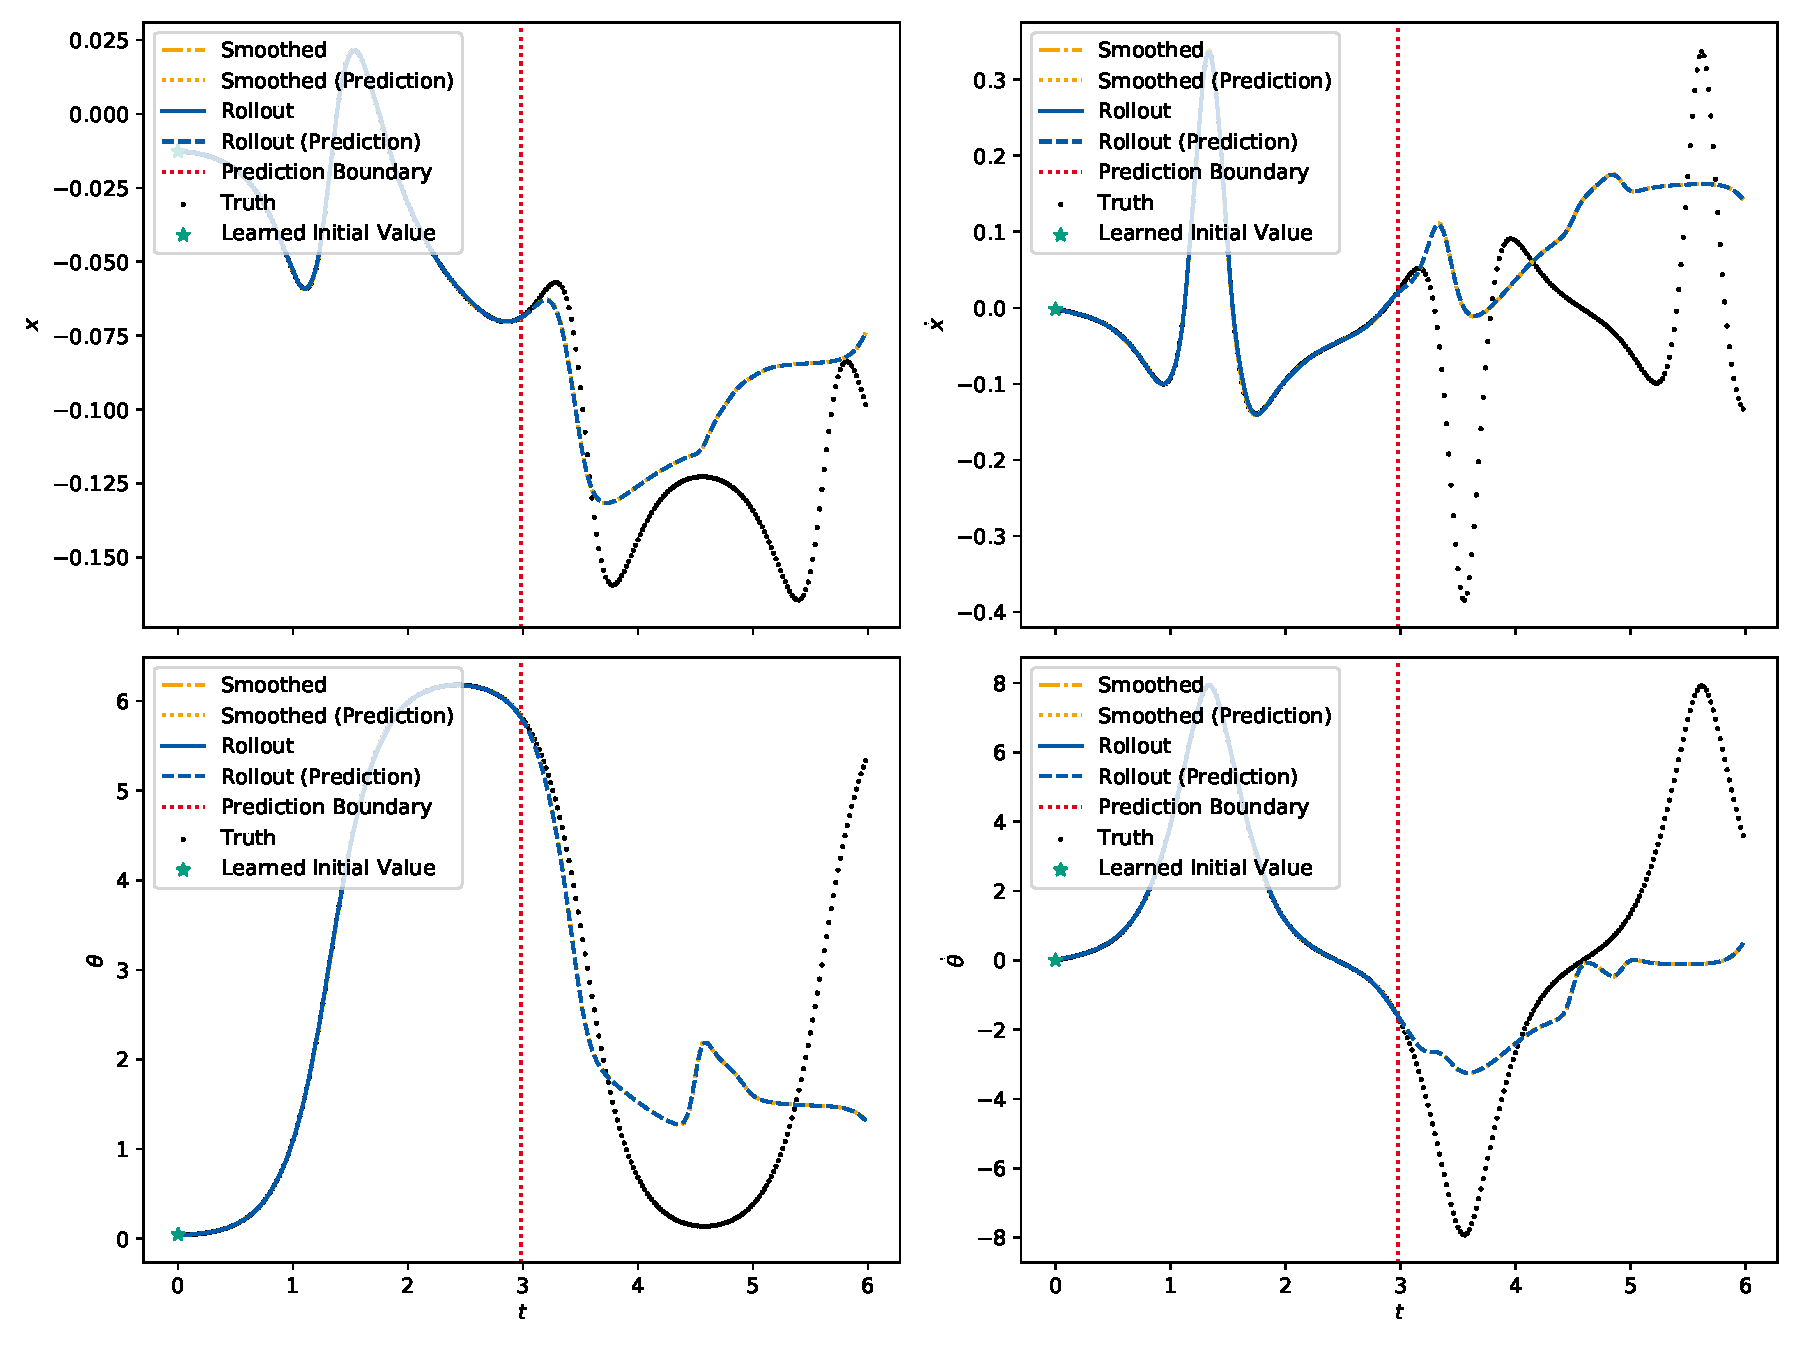
\includegraphics[width=\linewidth]{figures/results/cartpole-gym/run-latent-dim-16/without-confidence/rollout-observations-N0.pdf}
		\caption{This plot shows the same data as in~\autoref{fig:cartpoleRolloutL16}, but without the confidence shown.}
		\label{fig:cartpoleRolloutL16Appendix}
	\end{figure}
% end
